% Dont reinvent the wheel:
% http://journals.plos.org/ploscompbiol/article?id=10.1371/journal.pcbi.1002802
% http://www.jmlr.org/papers/volume8/sonnenburg07a/sonnenburg07a.pdf

% paper of Cox

\documentclass[twoside,11pt]{article} 
\usepackage{jmlr2e} 

\jmlrheading{}{}{}{}{}{Marc Claesen, Jaak Simm, Dusan Popovic, Yves Moreau and Bart De Moor}

\ShortHeadings{Optunity}{Claesen, Simm, Popovic, Moreau and De Moor}
\firstpageno{1}

\usepackage{amsmath}
\usepackage{tikz}
\usepackage{ifpdf}
\usepackage{multirow}
\usepackage{afterpage}
\usepackage{booktabs}
\usepackage{fancyvrb}
\usepackage{color}
\usepackage[colorlinks=false,allbordercolors={1 1 1}]{hyperref}
%\usepackage{url}
\usepackage{listings}
\usepackage{xspace}

%\usepackage{apacite}
\newcommand{\train}{\mathbf{X}^{(tr)}}
\newcommand{\test}{\mathbf{X}^{(te)}}
\newcommand{\obj}{\mathcal{F}}
\DeclareMathOperator*{\argmin}{arg\,min}

\definecolor{mygreen}{rgb}{0,0.6,0}
\definecolor{mygray}{rgb}{0.5,0.5,0.5}
\definecolor{bggray}{rgb}{0.95,0.95,0.95}
\definecolor{mymauve}{rgb}{0.58,0,0.82}
\lstdefinestyle{Py}{
    language={Python}, 
    moredelim=**[is][\slshape\bfseries]{`}{`},
    moredelim=**[is][\color{mygreen}]{!}{!},
}
\lstset{ %
%  backgroundcolor=\color{bggray},   % choose the background color; you must add \usepackage{color} or \usepackage{xcolor}
  basicstyle=\footnotesize\ttfamily, %\footnotesize,        % the size of the fonts that are used for the code
  breakatwhitespace=true,         % sets if automatic breaks should only happen at whitespace
  breaklines=true,                 % sets automatic line breaking
  captionpos=b,                    % sets the caption-position to bottom
  commentstyle=\color{mygray},    % comment style
  deletekeywords={...},            % if you want to delete keywords from the given language
  escapeinside={\%*}{*)},          % if you want to add LaTeX within your code
  extendedchars=true,              % lets you use non-ASCII characters; for 8-bits encodings only, does not work with UTF-8
  frame=single,                    % adds a frame around the code
  keepspaces=true,                 % keeps spaces in text, useful for keeping indentation of code (possibly needs columns=flexible)
  keywordstyle=\color{black},       % keyword style
  language=Python,                 % the language of the code
  morekeywords={svm\_acc, make\_solver, maximize},            % if you want to add more keywords to the set
  numbers=left,                    % where to put the line-numbers; possible values are (none, left, right)
  numbersep=5pt,                   % how far the line-numbers are from the code
  numberstyle=\tiny\color{mygray}, % the style that is used for the line-numbers
  rulecolor=\color{mygray},         % if not set, the frame-color may be changed on line-breaks within not-black text (e.g. comments (green here))
  showspaces=false,                % show spaces everywhere adding particular underscores; it overrides 'showstringspaces'
  showstringspaces=false,          % underline spaces within strings only
  showtabs=false,                  % show tabs within strings adding particular underscores
  stepnumber=1,                    % the step between two line-numbers. If it's 1, each line will be numbered
  stringstyle=\color{mymauve},     % string literal style
  tabsize=2,                       % sets default tabsize to 2 spaces
  title=\lstname,                   % show the filename of files included with \lstinputlisting; also try caption instead of title
  belowskip=0em,
  belowcaptionskip=-2em,
  columns=fullflexible,
  keepspaces=true
}
\renewcommand{\lstlistingname}{Snippet}


\hyphenation{Optunity}
\newcommand{\optunity}{{\sc Optunity}\xspace}

\begin{document}

\title{Easy Hyperparameter Search Using Optunity}

\author{\name Marc Claesen \email marc.claesen@esat.kuleuven.be  \\ 
\name Jaak Simm \email jaak.simm@esat.kuleuven.be   \\ 
\name Dusan Popovic \email dusan.popovic@esat.kuleuven.be   \\ 
\name Yves Moreau \email yves.moreau@esat.kuleuven.be \\
\name Bart De Moor \email bart.demoor@esat.kuleuven.be  \\ 
\addr KU Leuven, Department of Electrical Engineering (ESAT) \\
STADIUS Center for Dynamical Systems, Signal Processing and Data Analytics \\ 
iMinds, Department of Medical Information Technologies \\
Kasteelpark Arenberg 10, box 2446; 3001 Leuven, Belgium
}

\editor{TBD}

\maketitle

\begin{abstract}%   <- trailing '%' for backward compatibility of .sty file
    \optunity is a free software package dedicated to hyperparameter optimization. It contains various types of solvers, ranging from undirected methods to direct search, particle swarm and evolutionary optimization. The design focuses on ease of use, flexibility, code clarity and interoperability with existing software in popular machine learning environments. \optunity is written in Python and contains interfaces to R, Octave and MATLAB.  \optunity uses a BSD license and is available at \texttt{\url{http://www.optunity.net}}.
\end{abstract}

\begin{keywords}
  hyperparameter search, black-box optimization, algorithm tuning, Python
\end{keywords}

\section{Introduction}
Many machine learning tasks involve training a model $\mathcal{M}$ which minimizes some loss function $\mathcal{L}(\mathcal{M}\ |\ \test)$ on given test data $\test$. A model is obtained via a learning algorithm $\mathcal{A}$ which uses a training set $\train$ and solves some optimization problem. The learning algorithm $\mathcal{A}$ may itself be parameterized by a set of hyperparameters $\lambda$, e.g. $\mathcal{M} = \mathcal{A}(\train\ |\ \lambda)$.  Hyperparameter search -- also known as tuning -- aims to find a set of hyperparameters $\lambda^*$, such that the learning algorithm yields an optimal model $\mathcal{M}^*$ that minimizes $\mathcal{L}(\mathcal{M}\ |\ \test)$:
\begin{equation}
\lambda^* = \argmin_{\lambda} \mathcal{L}\big(\mathcal{A}(\train\ |\ \lambda)\ |\ \test\big) = \argmin_{\lambda} \obj(\lambda\ |\ \mathcal{A},\ \train, \test,\ \mathcal{L}). \label{equation}
\end{equation}
In tuning, $\obj$ is the objective function and the hyperparameters $\lambda$ are optimization variables. The learning algorithm $\mathcal{A}$, loss function $\mathcal{L}$ and data sets $\train$ and $\test$ are known. %Depending on the learning task, $\train$ and $\test$ may be labeled and/or equal to each other. The objective function often has a constrained domain (for example regularization terms must be positive) and is assumed to be expensive to evaluate, black-box and non-smooth.

Tuning hyperparameters is a recurrent task in machine learning which may significantly affect overall performance. Commonly tuned hyperparameters are related to kernels, regularization, learning rates and network architecture. Some specific challenges associated to hyperparameter optimization are discussed by \citet{claesen2015hyperparameter}. General machine learning packages provide only basic tuning methods like grid search \citep{pedregosa2011scikit}. In practice, the most common tuning approaches are grid search and manual tuning, though both are known to fail when the number of hyperparameters grows and manual search is additionally hard to reproduce \citep{bergstra2012random}.

\section{Optunity}
\optunity offers various optimizers and utility functions to enable efficient hyperparameter optimization using only a few of lines of code and minimal expertise. Our software is complementary to libraries that provide learning algorithms, such as \textsc{scikit-learn} \citep{pedregosa2011scikit}. The package uses a BSD license and is simple to deploy in any environment. \optunity supports Python, R, Octave and MATLAB on Linux, OSX and Windows.

\subsection{Functional Overview}
\optunity provides both simple routines for lay users and expert routines that enable fine-grained control of various aspects of the solving process. Basic tuning requires only an objective function, a maximum number of evaluations and box constraints on the hyperparameters to be optimized. Conditional search spaces in which the existence of some hyperparameters is contingent upon some discrete choice are also supported.

The objective function must be defined by the user. It takes a hyperparameter tuple $\lambda$ and typically involves three steps: (i) training a model $\mathcal{M}$ with $\lambda$, (ii) use $\mathcal{M}$ to predict a test set (iii) compute some score or loss based on the predictions. In unsupervised tasks, the separation between (i) and (ii) need not exist, for example in clustering a data set.

Tuning involves a series of function evaluations until convergence or until a predefined maximum number of evaluations is reached. \optunity is capable of vectorizing evaluations in the working environment to speed up the process at the end user's volition.

\optunity also provides $k$-fold cross-validation to estimate the generalization performance of supervised modeling approaches. The implementation can account for strata and clusters.\footnote{Instances in a stratum should be spread across folds. Clustered instances must remain in a single fold.} Finally, a variety of common quality metrics is available. 
The snippet below shows how to tune an SVM classifier with RBF kernel using {\sc scikit-learn} and \optunity:\footnote{We assume the correct imports are made and \texttt{data} and \texttt{labels} contain appropriate content.}

\begin{lstlisting}[style=Py, frame=none, xleftmargin=3.5ex, escapeinside={(*@}{@*)}, belowskip=-2.2\medskipamount]
!@optunity.cross_validated!(x=(*@\textcolor{red}{data}@*), y=(*@\textcolor{red}{labels}@*), num_folds=10, num_iter=2)
def (*@\textcolor{blue}{svm\_auc}@*)(x_train, y_train, x_test, y_test, (*@\textcolor{blue}{C}@*), (*@\textcolor{blue}{gamma}@*)):
    model = sklearn.svm.SVC(C=10**(*@\textcolor{blue}{C}@*), gamma=10**(*@\textcolor{blue}{gamma}@*)).fit(x_train, y_train)
    decision_values = model.decision_function(x_test)
    return !optunity.metrics.roc_auc!(y_test, decision_values)

!hps!, _, _ = !optunity.maximize!((*@\textcolor{blue}{svm\_auc}@*), num_evals=100, (*@\textcolor{blue}{C=[-5, 2]}@*), (*@\textcolor{blue}{gamma=[-5, 0]}@*)) (*@\label{optunity-maximize}@*)
svm = sklearn.svm.SVC(C=10**!hps['C']!, gamma=10**!hps['gamma']!).fit((*@\textcolor{red}{data}@*), (*@\textcolor{red}{labels}@*))
\end{lstlisting}
\ifx
%\newpage
\begin{lstlisting}[style=Py, frame=none, xleftmargin=3.5ex, escapeinside={(*@}{@*)}, belowskip=-2.2\medskipamount]
!@optunity.cross_validated!(x=(*@\textcolor{red}{data}@*), y=(*@\textcolor{red}{labels}@*), num_folds=10, num_iter=2)
def (*@\textcolor{blue}{svm\_auc}@*)(x_train, y_train, x_test, y_test, (*@\textcolor{blue}{C}@*), (*@\textcolor{blue}{gamma}@*)):
    model = sklearn.svm.SVC(C=(*@\textcolor{blue}{C}@*), gamma=(*@\textcolor{blue}{gamma}@*)).fit(x_train, y_train)
    decision_values = model.decision_function(x_test)
    return !optunity.metrics.roc_auc!(y_test, decision_values)

optimal_pars, _, _ = !optunity.maximize!((*@\textcolor{blue}{svm\_auc}@*), num_evals=100, (*@\textcolor{blue}{C=[0, 10]}@*), (*@\textcolor{blue}{gamma=[0, 1]}@*)) (*@\label{optunity-maximize}@*)
optimal_model = sklearn.svm.SVC(**optimal_pars).fit((*@\textcolor{red}{data}@*), (*@\textcolor{red}{labels}@*))
\end{lstlisting}
\fi

The objective function as per Equation~\eqref{equation} is defined on lines 1 to 5, where $\lambda = (C, \gamma)$, $\mathcal{A}$ is the SVM training algorithm and $\mathcal{L}$ is area under the ROC curve. We use $2\times$ iterated 10-fold cross-validation to estimate area under the ROC curve. Up to $100$ hyperparameter tuples are tested within the box constraints $10^{-5} < C < 10^2$ and $10^{-5} < \gamma < 10^0$ on line \ref{optunity-maximize}.


\subsection{Available Solvers}
\optunity provides a wide variety of solvers, ranging from basic, undirected methods like grid search, sobol sequences and random search \citep{bergstra2012random} to evolutionary methods such as particle swarm optimization \citep{kennedy2010particle}, the covariance matrix adaptation evolutionary strategy (CMA-ES) \citep{hansen2001completely}, tree-structured Parzen estimator \citep{bergstra2011algorithms} and the Nelder-Mead simplex. The default solver is particle swarm optimization, which performs well for a large variety of tuning tasks involving various learning algorithms. Additional solvers will be incorporated in the future.
 
\subsection{Software Design and Implementation}

The design philosophy of \optunity prioritizes code clarity over performance. This is justified by the fact that objective function evaluations constitute the performance bottleneck. 

In contrast to typical Python packages, we avoid dependencies to facilitate users working in non-Python environments (sometimes at the cost of performance). To prevent issues for users that are unfamiliar with Python, care is taken to ensure all code in \optunity works out of the box on any Python version above 2.7, without requiring tools like \texttt{2to3} to make explicit conversions. \optunity has dependencies on {\sc DEAP} \citep{fortin2012deap} and {\sc Hyperopt} \citep{bergstra2013hyperopt} for the CMA-ES and TPE solvers, respectively. 

A key aspect of \optunity's design is interoperability with external environments. This requires bidirectional communication between \optunity's Python back-end ($\mathcal{O}$) and the external environment ($\mathcal{E}$) and roughly involves three steps: (i) $\mathcal{E}\rightarrow\mathcal{O}$ solver configuration, (ii) $\mathcal{O}\leftrightarrow\mathcal{E}$ objective function evaluations and (iii) $\mathcal{O}\rightarrow\mathcal{E}$ solution and solver summary. To this end, \optunity can do straightforward communication with any environment via sockets using JSON messages as shown in Figure~\ref{fig:workflow}. Only some information must be communicated, big objects like data sets are never exchanged. To port \optunity to a new environment, a thin wrapper must be implemented to handle communication.

\begin{figure}[!h]
  \centering 
      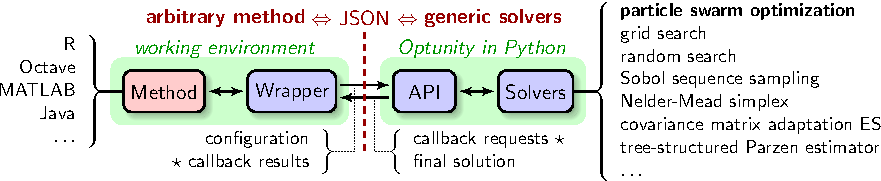
\includegraphics[width=\textwidth]{software.pdf} 
  \caption{Integrating \optunity in non-Python environments.}\label{fig:workflow}
\vspace{-1.5em}
\end{figure}

\subsection{Development and Documentation}
Collaborative development is organized via GitHub.\footnote{We maintain the following subdomains for convenience: \texttt{http://}$\{$\href{http://builds.optunity.net}{builds}, \href{http://docs.optunity.net}{docs}, \href{http://git.optunity.net}{git}, \href{http://issues.optunity.net}{issues}$\}$\texttt{.optunity.net}.} The project's master branch is kept stable and is subjected to continuous integration tests using Travis CI. 
We recommend prospective users to clone the master branch for the most up-to-date stable version of the software. Bug reports and feature requests can be filed via issues on GitHub. Future development efforts will focus on wrappers for Java and C/C++. We additionally plan to incorporate Bayesian optimizers which have no reference implementation in other packages. %Bayesian optimization strategies that are unavailable elsewhere \citep{jones1998efficient}. 

Code is documented using Sphinx and contains many doctests that can serve as both unit tests and examples of the associated functions. 
Our website contains API documentation, user documentation and a wide range of examples to illustrate all aspects of the software. 
The examples involve various packages and environments, including \textsc{scikit-learn} \citep{pedregosa2011scikit}, \textsc{OpenCV} and \textsc{Spark}'s \textsc{MLlib} \citep{zaharia2010spark}.
%Finally, some practical applications are available, including object recognition using OpenCV \citep{opencv_library} and deep learning with Theano \citep{bergstra2011theano}. % and semisupervised learning \citep{Claesen2015resvm}.

%\section{Conclusions}
%Optunity contains a variety of optimization methods that can be used for hyperparameter search. Using proper search methods becomes particularly important for machine learning methods with many hyperparameters, such as convolutional networks, deep belief networks and ensembles of SVM models.

\section{Related Work}

A number of software solutions exist for hyperparameter search. \textsc{Hyperopt} offers random search and sequential model-based optimization \citep{bergstra2013hyperopt}. Some packages dedicated to Bayesian approaches include \textsc{Spearmint} \citep{snoek2012practical}, \textsc{DiceKriging} \citep{roustant2012dicekriging}. Finally, \textsc{ParamILS} is a command-line-only tuning framework providing iterated local search \citep{hutter2009paramils}. 

%Existing packages tend to be one-trick ponies, providing a specific class of optimization methods and offering limited support to users in different machine learning environments. 
\optunity distinguishes itself from other packages by exposing a variety of fundamentally different solvers through a lightweight API. \optunity's client-server model facilitates integration in any language and environment and can even be used to run solvers remotely.

\ifx
\section{Solver Benchmark}
We compared our particle swarm optimization (PSO) solver against the tree of Parzen estimators (TPE) as is available in \textsc{Hyperopt \citep{bergstra2013hyperopt}. We tuned an SVM with elliptic RBF kernel $\kappa(\mathbf{u},\mathbf{v}) = \exp(-\gamma \|\mathbf{u}\beta - \mathbf{v}\beta\|^2)$ on a synthetic 3-D data set, where $\beta$ is a $3\times3$ diagonal matrix. The task involves optimizing $5$ hyperparameters: 4 kernel parameters ($\gamma$ and diagonal elements of $\beta$) and the misclassification penalty $C$. All solvers received a budget of $60$ evaluations and an identical search space. In each run, we generated train and test sets, optimized 10-fold cross-validated area under the ROC curve (AUROC) and computed test set AUROC. $\Delta$ denotes the difference in test set AUROC between one model and the best per run. The code for this simulation is available at \url{blah}.

Table~\ref{table:results} shows the results of $100$ runs. Both PSO and TPE outperform random search. PSO yielded the best set of hyperparameters most often for this tuning task (46/100). PSO features the lowest average rank and smallest maximum $\Delta$. %Since PSO has more wins than TPE but equal average $\Delta$, PSO is further behind the winner than TPE on average (when losing).

\begin{table}[!ht]
\centering
\begin{tabular}{lccccr}
\toprule
				&		&		& \multicolumn{3}{c}{test set AUROC ($\%$)} 	\\ \cline{4-6}
solver 				& wins 		& average rank 	&	average	& average $\Delta$ 	& max $\Delta$	\\
\midrule
random search			& 23 		& 2.20		& 73.54		& 2.76			& 13.38 \\
PSO				& \textbf{46} 	& \textbf{1.77} & 74.52 	& 1.78			& \textbf{9.50} \\
TPE				& 31		& 2.03		& \textbf{74.53}& \textbf{1.77}		& 10.37 \\
\bottomrule
\end{tabular}
\caption{Benchmark results: number of wins (best test set AUROC), average rank per approach (lower is better) and test set performance (lower $\Delta$ is better).} 
\label{table:results}
\end{table}
\fi

\section{Solver Performance Benchmark}
\textsc{Optunity}'s particle swarm optimizer (PSO) was compared to \textsc{Hyperopt}'s tree of Parzen estimators (TPE) in minimizing the Rastrigin function $f(x, y) = 20 + x^2 - 10 \cos(2\pi x) + y^2 - 10 \cos(2\pi y)$, which has a known optimum $f(0,0)=0$.
%\begin{equation}
%f(x, y) = 20 + x^2 - 10 \cos(2\pi x) + y^2 - 10 \cos(2\pi y), \quad \text{optimum: } f(0, 0) = 0 \label{eq:rastrigin},
%\end{equation}
Optimization was done uniformly within box constraints $|x|, |y| < 5.12$. We used the Rastrigin function because it has many local minima, as is common in hyperparameter search \citep{claesen2015hyperparameter}. Figure~\ref{fig:benchmark} shows that both PSO and TPE outperform random search. TPE is marginally better than PSO initially (few evaluations) while PSO converges much faster later on. PSO has also been shown to be competitive to TPE in tuning RBMs by \citet{papa2015model}.

\begin{figure}[!h]
  \centering 
      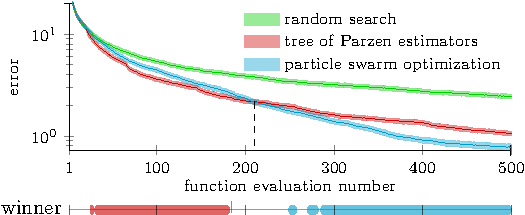
\includegraphics[width=0.65\textwidth]{benchmark.pdf} \ \ 
      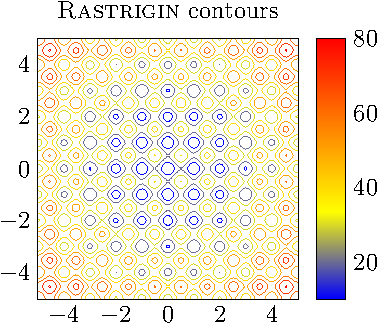
\includegraphics[width=0.32\textwidth]{rastrigin.pdf}\vfill
  \caption{Evolution of average error per solver while minimizing the \textsc{Rastrigin} function (contours depicted on the right) based on 1,000 repetitions. The winner line shows the statistically significant best solver per evaluation count, if any ($\alpha=5\%$).}\label{fig:benchmark}
\vspace{-3em}
\end{figure}


\acks{This research was funded via the following channels: Research Council KU Leuven: GOA/10/09 MaNet, CoE PFV/10/016 SymBioSys; Flemish Government: FWO: projects:  G.0871.12N (Neural circuits); IWT: TBM-Logic Insulin(100793), TBM Rectal Cancer(100783), TBM IETA(130256), O\&O ExaScience Life Pharma, ChemBioBridge, PhD grants (specifically 111065); Industrial Research fund (IOF): IOF/HB/13/027 Logic Insulin; iMinds Medical IT SBO 2014; VLK Stichting E. van der Schueren: rectal cancer; Federal Government: FOD: Cancer Plan 2012-2015 KPC-29-023 (prostate).}

\newpage
\bibliography{bibliography}

\end{document}
